%% Le lingue utilizzate, che verranno passate come opzioni al pacchetto babel. Come sempre, l'ultima indicata sar� quella primaria.
%% Se si utilizzano una o pi� lingue diverse da "italian" o "english", leggere le istruzioni in fondo.
\def\thudbabelopt{english,italian}
%% Valori ammessi per target: bach (tesi triennale), mst (tesi magistrale), phd (tesi di dottorato).
%% Valori ammessi per aauheader: '' (vuoto -> nessun header Alpen Adria Univeristat), aics (Department of Artificial Intelligence and Cybersecurity), informatics (Department of Informatics Systems). Il nome del dipartimento � allineato con la versione inglese del logo UniUD.
\documentclass[target=bach,aauheader=]{thud}

%% --- Informazioni sulla tesi ---
%% Per tutti i tipi di tesi
% Scommentare quello di interesse, o mettete quello che vi pare
\course{Informatica}
%\course{Internet of Things, Big Data e Web}
%\course{Matematica}
%\course{Comunicazione Multimediale e Tecnologie dell'Informazione}
\title{Interfacce utente per la selezione \\ di item nel contesto di video giochi \\ in realtà virtuale immersiva}
\author{Paolo Casagrande}
\supervisor{Dott.\ Fabio Buttussi}
%\cosupervisor{Arch.\ Rambaldo Melandri \and Dott.\ Giorgio Perozzi}
%\tutor{Guido Necchi}
%% Campi obbligatori: \title, \author e \course.
%% Altri campi disponibili: \reviewer, \tutor, \chair, \date (anno accademico, calcolato in automatico), \rights
%% Con \supervisor, \cosupervisor, \reviewer e \tutor si possono indicare pi� nomi separati da \and.
%% Per le sole tesi di dottorato:
%\phdnumber{313}
%\cycle{XXVIII}
%\contacts{Via della Sintassi Astratta, 0/1\\65536 Gigatera --- Italia\\+39 0123 456789\\\texttt{http://www.example.com}\\\texttt{inbox@example.com}}

%% --- Pacchetti consigliati ---
%% pdfx: per generare il PDF/A per l'archiviazione. Necessario solo per la versione finale
\usepackage[a-1b]{pdfx}
%% hyperref: Regola le impostazioni della creazione del PDF... pi� tante altre cose. Ricordarsi di usare l'opzione pdfa.
\usepackage[pdfa]{hyperref}
%% tocbibind: Inserisce nell'indice anche la lista delle figure, la bibliografia, ecc.

%% --- Stili di pagina disponibili (comando \pagestyle) ---
%% sfbig (predefinito): Apertura delle parti e dei capitoli col numero grande; titoli delle parti e dei capitoli e intestazioni di pagina in sans serif.
%% big: Come "sfbig", solo serif.
%% plain: Apertura delle parti e dei capitoli tradizionali di LaTeX; intestazioni di pagina come "big".

% package per le immagini
\usepackage{graphicx}
\graphicspath{ {./images/} }

\begin{document}
\maketitle

%% Dedica (opzionale)
%\begin{dedication}
%	Al mio cane,\par per avermi ascoltato mentre ripassavo le lezioni.
%\end{dedication}

%% Ringraziamenti (opzionali)
\acknowledgements
Speriamo bene
%% Sommario (opzionale)
%\abstract
%Nunc ac dignissim ipsum, quis pulvinar elit. Mauris congue nec leo ornare lobortis. Nulla hendrerit pretium diam nec lobortis. Nullam aliquam laoreet nisl, sit amet facilisis lectus accumsan ut. Duis et elit hendrerit metus venenatis condimentum. Integer id eros molestie, interdum leo sit amet, aliquet metus. Integer fermentum tristique magna, vel luctus neque rhoncus vel. Ut hendrerit et quam et semper. Mauris egestas, odio sed aliquet luctus, magna orci euismod odio, vitae lacinia tellus tellus non lectus. Aliquam urna neque, porta et mattis aliquam, congue sit amet lorem. In ultrices augue sit amet ante vehicula, vitae rhoncus turpis auctor. Donec porta scelerisque eros, at mollis enim imperdiet ut. 

%% Indice
\tableofcontents

%% Lista delle tabelle (se presenti)
%\listoftables

%% Lista delle figure (se presenti)
%\listoffigures

%% Corpo principale del documento
\mainmatter

%% Parte
%% La suddivisione in parti � opzionale; solitamente sono sufficienti i capitoli.
%\part{Parte}
%\nocite{*} %% rimuovere magari in seguito
%% Capitolo
\chapter{Introduzione} % Introduzione alla VR + Intro dispositivi + Intro capitoli
La Realtà Virtuale (Virtual Reality, VR) è un'interfaccia avanzata uomo-computer che simula un ambiente realistico \cite{Zheng}.
All'interno di questo ambiente l'utente è libero di muoversi, esplorare ed interagire con qualsiasi cosa, alimentando la sensazione di sentirsi effettivamente presente all'interno di un mondo virtuale.
Al giorno d'oggi, la Realtà Virtuale può essere applicata a vari settori tra cui l'intrattenimento, l'educazione, medico e commerciale. \\

L'interazione tra uomo e ambiente virtuale avviene attraverso specifici dispositivi.
L'interfaccia avanzata più utilizzata nella Realtà Virtuale è il visore VR. 
Questo visore, denominato \textit{Head Mounted Dispaly}, può essere indossato come un casco che mostra all'utente il mondo virtuale a 360°.
Il visore VR utilizzato per l'esperimento è il Visore VR HTC Vive Pro, visibile in figura \ref{fig:vive_pro}.

\begin{figure}[h]
    \centering
    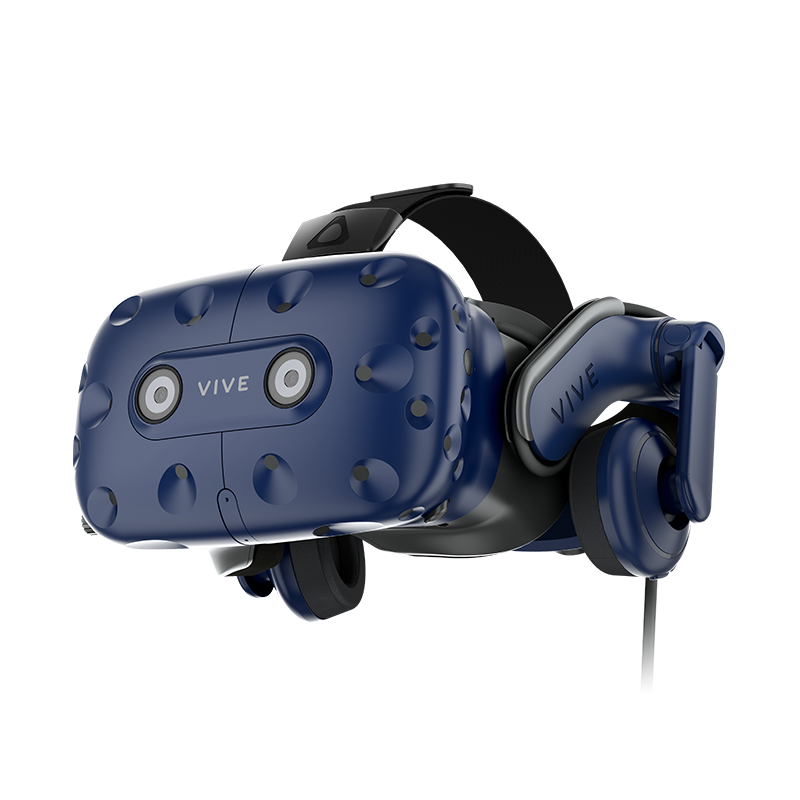
\includegraphics[width=0.25\textwidth]{vive_pro}
    \caption{Visore VR HTC Vive Pro}
    \label{fig:vive_pro}
\end{figure}

Insieme al visore, per interagire all'interno dell'ambiente virtuale, l'utente utilizza una coppia di controller per muovere entrambe le mani \ref{fig:vive_contr}.
Questi controller mappano il movimento delle mani nello spazio reale, che viene poi rappresentato nel mondo virtuale. 
L'utente può premere i tasti sui controller per esercitare azioni specifiche che interagiscono con l'ambiente virtuale. \\

\begin{figure}[h]
    \centering
    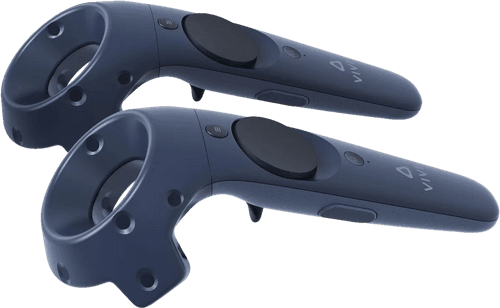
\includegraphics[width=0.25\textwidth]{vive_contr}
    \caption{Controller per HTC Vive Pro}
    \label{fig:vive_contr}
\end{figure}

\newpage
L'obiettivo della tesi è quello di sviluppare un'interfaccia virtuale efficace che permetta agli utenti di selezionare determinati item.
L'efficacia dell'interfaccia dipenderà dalla facilità di selezione di un item, dalla rapidità con la quale lo si seleziona e dalla fatica che bisogna fare per selezionarlo.
Sono state progettate molte interfacce, come verrà spiegato meglio nei prossimi capitoli, per ottenere le due interfacce finali migliori. \\


Nel capitolo 2 viene descritto lo stato dell'arte riguardante la Realtà Virtuale e alcuni studi riguardo a interfacce in ambienti virtuali.
Nel capitolo 3 si spiega la programmazione dell'ambiente virtuale, nel capitolo 4 come sono state progettate tutte le interfacce.
Nel capitolo 5 vengono poi confrontate le interfacce più efficaci, mentre nel capitolo 6 si conclude la tesi parlando di ulteriori sviluppi futuri.
%% Sezione
%\section{Titolo della Sezione}

%% Sottosezione
%\subsection{Sottosezione}

\chapter{Stato dell'arte} % Studi VR e interfacce + Legame tra VR e dispositivi
\section{VR e interfacce immersive}
Esistono molti studi che comparano diverse interfacce immersive per interagire nelle applicazioni VR.
Ad esempio, uno studio condotto da Daniel Hepperle et al.\cite{Hepperle} ha confrontato tre diverse interfacce - 2D, 3D e a comando vocale - per capire quale fosse la migliore per la Realtà Virtuale.  
Nello studio sono stati coinvolti 30 partecipanti, di cui 20 maschi e 10 femmine.
Degli utenti, solo il 66\% aveva esperienza con sistemi VR e il 50\% aveva già usato un dispositivo 3D prima d'ora.
La prova consisteva nel completare 17 compiti con le 3 interfacce nel minor tempo possibile e infine compilare un questionario.
I compiti comprendevano selezione, manipolazione, creazione, rotazione e modifica di oggetti virtuali.
Dai risultati è emerso che gli utenti, usando l'interfaccia sviluppata in 3D, consideravano l'input intuitivo e naturale; inoltre, rispetto alle altre interfacce, si sentivano più immersi nell'attività. \\

Uno studio di Rennan Raffaele et al.\cite{Raffaele} ha analizzato quale interfaccia immersiva fosse la migliore nei giochi VR.
Le interfacce a confronto proponevano rappresentazione spaziale, diegetica e non-diegetica.
Allo studio hanno partecipato 50 utenti, che spaziavano tra designer, sviluppatori e videogiocatori.
I partecipanti dovevano infine compilare un questionario che paragonava 16 interfacce diverse utilizzate nei videogiochi.
I risultati hanno mostrato che la rappresentazione diegetica è quella che permette la maggiore immersività di un'interfaccia in un ambiente virtuale.



https://www.hindawi.com/journals/ijcgt/2018/3757083/ \\ %% good gaming interface
https://dl.acm.org/doi/abs/10.1145/1536513.1536559 \\ %% rotto
http://gamescriticism.org/articles/schmalzer-4-1 \\ %% tanto



\section{Pedana}

\section{Visore}

\chapter{Progettazione dell'ambiente} % Spiegazione livello e menu vari + periferiche


\chapter{Design delle interfacce} % Percorso per arrivare alle interfacce adatte

\chapter{Discussione}

\chapter{Conclusioni} % cosa si può fare

%% Fine dei capitoli normali, inizio dei capitoli-appendice (opzionali)
%\appendix
%\part{Appendici}
%\chapter{Titolo della prima appendice}

%% Parte conclusiva del documento; tipicamente per riassunto, bibliografia e/o indice analitico.
\backmatter

%% Riassunto (opzionale)
%\summary
%Maecenas tempor elit sed arcu commodo, dapibus sagittis leo egestas. Praesent at ultrices urna. Integer et nibh in augue mollis facilisis sit amet eget magna. Fusce at porttitor sapien. Phasellus imperdiet, felis et molestie vulputate, mauris sapien tincidunt justo, in lacinia velit nisi nec ipsum. Duis elementum pharetra lorem, ut pellentesque nulla congue et. Sed eu venenatis tellus, pharetra cursus felis. Sed et luctus nunc. Aenean commodo, neque a aliquam bibendum, mauris augue fringilla justo, et scelerisque odio mi sit amet diam. Nulla at placerat nibh, nec rutrum urna. Donec ut egestas magna. Aliquam erat volutpat. Phasellus vestibulum justo sed purus mattis, vitae lacinia magna viverra. Nulla rutrum diam dui, vel semper mi mattis ac. Vestibulum ante ipsum primis in faucibus orci luctus et ultrices posuere cubilia Curae; Donec id vestibulum lectus, eget tristique est.

%% Bibliografia (praticamente obbligatoria)
\bibliographystyle{plain_\languagename}%% Carica l'omonimo file .bst, dove \languagename � la lingua attiva.
%% Nel caso in cui si usi un file .bib (consigliato)
\bibliography{thud}
%% Nel caso di bibliografia manuale, usare l'environment thebibliography.

%% Per l'indice analitico, usare il pacchetto makeidx (o analogo).

\end{document}

--- Istruzioni per l'aggiunta di nuove lingue ---
Per ogni nuova lingua utilizzata aggiungere nel preambolo il seguente spezzone:
    \addto\captionsitalian{%
        \def\abstractname{Sommario}%
        \def\acknowledgementsname{Ringraziamenti}%
        \def\authorcontactsname{Contatti dell'autore}%
        \def\candidatename{Candidato}%
        \def\chairname{Direttore}%
        \def\conclusionsname{Conclusioni}%
        \def\cosupervisorname{Co-relatore}%
        \def\cosupervisorsname{Co-relatori}%
        \def\cyclename{Ciclo}%
        \def\datename{Anno accademico}%
        \def\indexname{Indice analitico}%
        \def\institutecontactsname{Contatti dell'Istituto}%
        \def\introductionname{Introduzione}%
        \def\prefacename{Prefazione}%
        \def\reviewername{Controrelatore}%
        \def\reviewersname{Controrelatori}%
        %% Anno accademico
        \def\shortdatename{A.A.}%
        \def\summaryname{Riassunto}%
        \def\supervisorname{Relatore}%
        \def\supervisorsname{Relatori}%
        \def\thesisname{Tesi di \expandafter\ifcase\csname thud@target\endcsname Laurea\or Laurea Magistrale\or Dottorato\fi}%
        \def\tutorname{Tutor aziendale}%
        \def\tutorsname{Tutor aziendali}%
    }
sostituendo a "italian" (nella 1a riga) il nome della lingua e traducendo le varie voci.